%!TEX root = ../Thesis.tex
\section{Step 1}
The system given has the cars driving around the circuit in their specific routes. The cars does not stop, when they bump into each other, instead a red square is shown for each collision.
\\

Step one's requirements are to
\begin{itemize}
\item make sure the cars do not collide
\item cause deadlocks in the traffic
\item have cars drive through the alley
\end{itemize}



\begin{figure}[H]
\centering
\caption{The cars driving around the parking lot}
\begin{subfigure}[b]{0.4\textwidth}
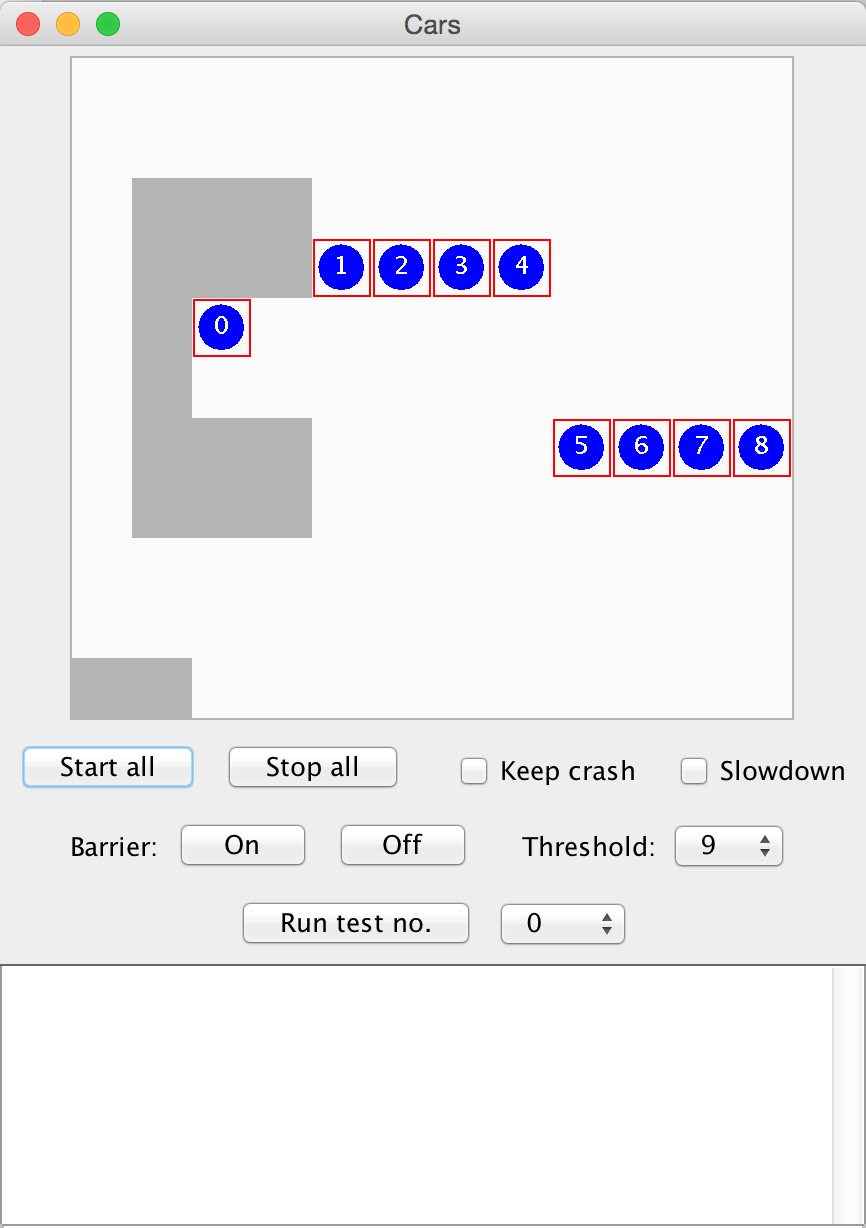
\includegraphics[scale=0.3]{./graphics/Cars1.png}
\end{subfigure}
\begin{subfigure}[b]{0.4\textwidth}
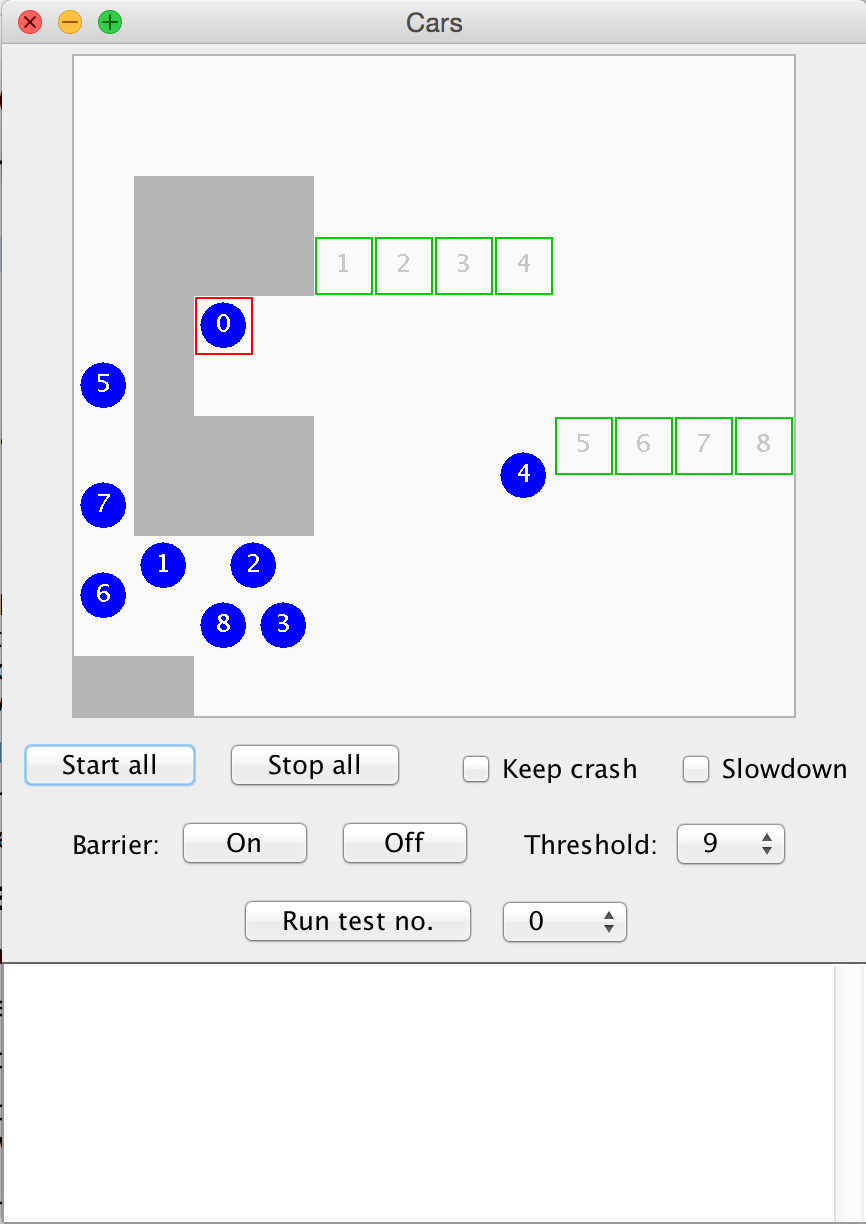
\includegraphics[scale=0.3]{./graphics/Cars2.png}
\end{subfigure}

\end{figure}